\documentclass[11pt]{article}
\usepackage[margin=1in]{geometry}
\usepackage{amsmath,amssymb,amsthm}
\usepackage{booktabs}
\usepackage{graphicx}
\usepackage{float}
\usepackage{enumitem}
\usepackage[hidelinks]{hyperref}

\newtheorem{theorem}{Theorem}
\theoremstyle{definition}
\newtheorem{definition}{Definition}

\newcommand{\R}{\mathbb{R}}
\newcommand{\checked}[2]{\par\smallskip\noindent\textit{Written by: #1. \quad Checked by: #2.}\par}
\graphicspath{{../figures/}{figures/}}

\title{Movie Recommender with Matrix Factorization\\[2pt]\large Iteration 2: The Math}
\author{Hakim Badmus \and Doyin Okwesa}
\date{\today}

\begin{document}
\maketitle

\section{Notation and Definitions}

\subsection{Notation}
\begin{center}\small
\begin{tabular}{lll}
\toprule
Symbol & Meaning & Size\\
\midrule
$m$ & number of users (943) & number\\
$n$ & number of movies (1682) & number\\
$k$ & number of hidden factors & number\\
$R$ & rating matrix; $r_{ui}$ is user $u$'s rating of movie $i$ & $m\times n$\\
$\Omega$ & the set of pairs $(u,i)$ where we know the rating & set\\
$U$ & user matrix; row $u$ is the vector $\mathbf u_u$ & $m\times k$\\
$V$ & movie matrix; row $i$ is the vector $\mathbf v_i$ & $n\times k$\\
$\mathbf u_u$ & what user $u$ likes & $k\times1$\\
$\mathbf v_i$ & what movie $i$ is like & $k\times1$\\
$\hat r_{ui}$ & predicted rating, $\mathbf u_u^\top\mathbf v_i$ & number\\
$n_u$ & number of movies user $u$ rated & number\\
$V_u$ & the rows of $V$ for the movies user $u$ rated & $n_u\times k$\\
$\mathbf r_u$ & the ratings user $u$ gave (same order as $V_u$) & $n_u\times1$\\
$\lambda$ & regularization strength, $\lambda>0$ & number\\
$J(U,V)$ & the objective we minimize & number\\
$I$ & identity matrix & $k\times k$\\
\bottomrule
\end{tabular}
\end{center}

\subsection{What the data means}
\begin{itemize}[nosep]
\item One \textbf{row} of $R$ is one user and all their ratings.
\item One \textbf{column} of $R$ is one movie and all the ratings it got.
\item One \textbf{entry} $r_{ui}$ is a star rating from 1 to 5. Most entries are blank because most users have not seen most movies.
\item One line of the data file is one known rating: (user, movie, rating, time).
\end{itemize}
The idea: each user and each movie gets a short vector of $k$ numbers. If they point in a similar direction, the dot product $\mathbf u_u^\top\mathbf v_i$ is big, and we predict a high rating.

\subsection{Definitions}
\begin{definition}[Norms]
For a vector, $\|\mathbf x\|^2=\mathbf x^\top\mathbf x=\sum_j x_j^2$. For a matrix, the Frobenius norm is $\|A\|_F^2=\sum_{i,j}a_{ij}^2$, which is the same as adding up $\|\text{row}\|^2$ over all rows.
\end{definition}

\begin{definition}[Positive definite]
A square matrix $A$ is \emph{positive semi-definite} if $\mathbf x^\top A\mathbf x\ge0$ for every $\mathbf x$, and \emph{positive definite} if $\mathbf x^\top A\mathbf x>0$ for every $\mathbf x\neq\mathbf 0$.
\end{definition}

\begin{definition}[Invertible]
A square matrix $A$ is invertible exactly when $A\mathbf x=\mathbf 0$ has only the solution $\mathbf x=\mathbf 0$ (Invertible Matrix Theorem).
\end{definition}

\begin{definition}[Gradient rules]
For a vector $\mathbf b$ and a symmetric matrix $A$:
$\nabla(\mathbf x^\top\mathbf b)=\mathbf b$ and $\nabla(\mathbf x^\top A\mathbf x)=2A\mathbf x$.
\end{definition}

\begin{definition}[Rank and SVD]
The rank of a matrix is the number of independent columns. Every matrix can be written as $A=W\Sigma Z^\top$ (the SVD), with singular values $\sigma_1\ge\sigma_2\ge\dots\ge0$. Keeping only the first $k$ pieces gives $A_k$, the truncated SVD.
\end{definition}

\begin{definition}[RMSE]
On a set $T$ of test ratings, $\text{RMSE}=\sqrt{\frac{1}{|T|}\sum_{(u,i)\in T}(r_{ui}-\hat r_{ui})^2}$. Lower is better. An RMSE of 1 means we are off by about 1 star.
\end{definition}

\begin{definition}[Normal distribution]
$x\sim\mathcal N(\mu,\sigma^2)$ has density $\propto\exp\!\big(-\frac{(x-\mu)^2}{2\sigma^2}\big)$.
\end{definition}
\checked{Hakim Badmus}{Doyin Okwesa}

\section{Assumptions}
\begin{enumerate}[label=\textbf{A\arabic*.}, leftmargin=*]
\item \textbf{A few factors explain most tastes} (low rank).
\emph{If false:} no small $k$ fits well, so errors stay high.
\emph{Check:} try several $k$ and plot test RMSE.

\item \textbf{Missing ratings are missing at random.}
\emph{If false:} people mostly rate movies they chose to watch, so known ratings lean high and our test score looks better than it really is.
\emph{Check:} compare RMSE on popular movies vs.\ rarely rated movies.

\item \textbf{Noise is random with mean 0 and the same size everywhere.}
\emph{If false:} squared error is not the right thing to minimize, and the probability result in Section 4 no longer holds.
\emph{Check:} histogram of test errors $r_{ui}-\hat r_{ui}$.

\item \textbf{$\lambda>0$.}
\emph{If false:} a user with fewer than $k$ ratings makes $V_u^\top V_u$ non-invertible, so the update in Q2 breaks.
\emph{Check:} pick $\lambda$ using a validation set.

\item \textbf{Every user and movie has at least one training rating.}
\emph{If false:} that user's vector becomes $\mathbf 0$ and every prediction for them is 0 stars (the ``cold start'' problem).
\emph{Check:} count users and movies missing from the training set.

\item \textbf{No built-in user or movie bias.} The model has no ``this user rates everything high'' term.
\emph{If false:} predictions get pulled toward 0, far below the average rating of about 3.5.
\emph{Fix:} subtract the average rating before training and add it back after (Step 0 of the algorithm).
\end{enumerate}
\checked{Doyin Okwesa}{Hakim Badmus}

\section{Iteration 2 -- Math Questions}

\subsection*{Q1. Write the objective}
We want $\mathbf u_u^\top\mathbf v_i$ to be close to $r_{ui}$, but only for ratings we actually know:
\[
J(U,V)=\sum_{(u,i)\in\Omega}\big(r_{ui}-\mathbf u_u^\top\mathbf v_i\big)^2+\lambda\big(\|U\|_F^2+\|V\|_F^2\big).
\]
\begin{itemize}[nosep]
\item The first part is the squared error on known ratings. Blank entries are skipped.
\item The second part keeps the numbers in $U$ and $V$ small, so the model does not memorize noise.
\end{itemize}
\textbf{Splitting $J$ by user.} Group the sum by user, and use $\|U\|_F^2=\sum_u\|\mathbf u_u\|^2$ (definition of Frobenius norm):
\[
J=\sum_{u=1}^m\underbrace{\Big[\sum_{i\text{ rated by }u}(r_{ui}-\mathbf v_i^\top\mathbf u_u)^2+\lambda\|\mathbf u_u\|^2\Big]}_{J_u(\mathbf u_u)}+\lambda\|V\|_F^2 .
\]
If $V$ is fixed, each $\mathbf u_u$ only shows up in its own $J_u$. So we can solve for each user on their own. The same is true for movies when $U$ is fixed.
\checked{Hakim Badmus}{Doyin Okwesa}

\subsection*{Q2. Solve for one user}
\begin{theorem}
If $V$ is fixed and $\lambda>0$, the best $\mathbf u_u$ is
\[
\mathbf u_u=(V_u^\top V_u+\lambda I)^{-1}V_u^\top\mathbf r_u .
\]
\end{theorem}
\begin{proof}
Write the sum of squares as a vector length, then expand.
\begin{align*}
J_u&=\|\mathbf r_u-V_u\mathbf u_u\|^2+\lambda\|\mathbf u_u\|^2 && \text{[sum of squares $=\|\cdot\|^2$]}\\
&=(\mathbf r_u-V_u\mathbf u_u)^\top(\mathbf r_u-V_u\mathbf u_u)+\lambda\,\mathbf u_u^\top\mathbf u_u && \text{[$\|\mathbf x\|^2=\mathbf x^\top\mathbf x$]}\\
&=\mathbf r_u^\top\mathbf r_u-2\,\mathbf u_u^\top V_u^\top\mathbf r_u+\mathbf u_u^\top V_u^\top V_u\mathbf u_u+\lambda\,\mathbf u_u^\top\mathbf u_u && \text{[multiply out]}\\
&=\mathbf r_u^\top\mathbf r_u-2\,\mathbf u_u^\top V_u^\top\mathbf r_u+\mathbf u_u^\top A\,\mathbf u_u && \text{[let $A=V_u^\top V_u+\lambda I$]}
\end{align*}
In the third line the two middle terms combined because $\mathbf r_u^\top V_u\mathbf u_u$ is a number, so it equals its own transpose $\mathbf u_u^\top V_u^\top\mathbf r_u$.
$A$ is symmetric because $(V_u^\top V_u)^\top=V_u^\top V_u$. Now take the gradient and set it to zero:
\begin{align*}
\nabla J_u&=-2V_u^\top\mathbf r_u+2A\,\mathbf u_u && \text{[gradient rules]}\\
0&=-2V_u^\top\mathbf r_u+2A\,\mathbf u_u && \text{[minimum: gradient is zero]}\\
A\,\mathbf u_u&=V_u^\top\mathbf r_u && \text{[rearrange: the normal equations]}\\
\mathbf u_u&=A^{-1}V_u^\top\mathbf r_u && \text{[$A$ is invertible, Q3]}
\end{align*}
This is a minimum and not a maximum: the second derivative is $2A$, which is positive definite (Q3), so $J_u$ is a bowl shape with exactly one lowest point.
\end{proof}
\noindent\textbf{In plain words:} this is ridge regression. The user's ratings are the $y$ values, the vectors of the movies they rated are the $x$ values, and $\mathbf u_u$ is the coefficient vector. For movies, swap the roles: $\mathbf v_i=(U_i^\top U_i+\lambda I)^{-1}U_i^\top\mathbf r_i$.
\checked{Hakim Badmus}{Doyin Okwesa}

\subsection*{Q3. $V_u^\top V_u+\lambda I$ is positive definite}
\begin{theorem}
For $\lambda>0$, $A=V_u^\top V_u+\lambda I$ is positive definite, so it is invertible.
\end{theorem}
\begin{proof}
Pick any $\mathbf x\neq\mathbf 0$.
\begin{align*}
\mathbf x^\top A\,\mathbf x&=\mathbf x^\top V_u^\top V_u\mathbf x+\lambda\,\mathbf x^\top\mathbf x && \text{[distribute]}\\
&=(V_u\mathbf x)^\top(V_u\mathbf x)+\lambda\,\mathbf x^\top\mathbf x && \text{[$(BC)^\top=C^\top B^\top$]}\\
&=\|V_u\mathbf x\|^2+\lambda\|\mathbf x\|^2 && \text{[$\mathbf y^\top\mathbf y=\|\mathbf y\|^2$]}\\
&>0 && \text{[first part $\ge0$; second part $>0$ since $\lambda>0$, $\mathbf x\ne\mathbf 0$]}
\end{align*}
So $A$ is positive definite. Now suppose $A\mathbf x=\mathbf 0$. Then $\mathbf x^\top A\mathbf x=0$, which only happens when $\mathbf x=\mathbf 0$. So $A$ is invertible (Invertible Matrix Theorem).
\end{proof}
\noindent\textbf{Extra fact:} the same steps show $\mathbf x^\top A\mathbf x\ge\lambda\|\mathbf x\|^2$, so every eigenvalue of $A$ is at least $\lambda$. We check this in the simulation.\\
\textbf{Why $\lambda$ matters:} without it, a user who rated fewer than $k$ movies gives a $V_u^\top V_u$ that cannot be inverted.
\checked{Hakim Badmus}{Doyin Okwesa}

\subsection*{Q4. ALS never makes $J$ worse}
ALS repeats two steps: (1) fix $V$, solve for every user with Q2; (2) fix $U$, solve for every movie the same way.
\begin{theorem}
After each step, $J$ is less than or equal to what it was before.
\end{theorem}
\begin{proof}
\textbf{User step.} From Q1, with $V$ fixed, $J$ is a sum of separate pieces $J_u(\mathbf u_u)$ plus a constant. Q2 gives the lowest possible value of each $J_u$. The lowest value is never more than the value at the old $\mathbf u_u$ [definition of minimum]. So each piece goes down or stays the same, and so does their sum.\\
\textbf{Movie step.} Same argument with users and movies swapped.\\
\textbf{Together:} $J_{\text{after}}\le J_{\text{middle}}\le J_{\text{before}}$.\\
\textbf{It settles down:} $J$ is made of squares, so $J\ge0$. A sequence that keeps going down but cannot go below 0 must level off [monotone convergence theorem].
\end{proof}
\noindent\textbf{Note:} this shows $J$ levels off, not that it reaches the best possible value. ALS can get stuck in a local minimum. Also, many different $U,V$ give the same $UV^\top$, so we compare $UV^\top$ to the truth, not $U$ itself.
\checked{Doyin Okwesa}{Hakim Badmus}

\subsection*{Q5. Why the SVD works for a full matrix but not with missing ratings}
\textbf{Eckart--Young theorem.} If every entry of $R$ is known, the truncated SVD $R_k$ is the best rank-$k$ approximation: no other rank-$k$ matrix $B$ has a smaller $\|R-B\|_F^2$. So for a full matrix, the SVD solves the problem directly with no iteration.

\textbf{The problem with missing ratings.} The SVD needs a full matrix, so the simple fix is to fill the blanks with 0. Split the error into known and blank entries:
\[
\|R_{\text{filled}}-B\|_F^2=\underbrace{\sum_{\text{known}}(r_{ui}-b_{ui})^2}_{\text{what we want}}+\underbrace{\sum_{\text{blank}}(0-b_{ui})^2}_{\text{extra penalty}} .
\]
The SVD minimizes this whole thing. The second part punishes any non-zero prediction for a movie the user has not seen. In MovieLens about 94\% of entries are blank, so this part dominates and the SVD learns to predict about 0 stars for unseen movies. That is the opposite of what we want.

ALS only uses the first part, which is why it does better. That objective has no closed-form answer, which is why we need to iterate.

\textbf{Small example.} Take $R=\begin{pmatrix}1&?\\1&1\end{pmatrix}$ and $k=1$.
\begin{itemize}[nosep]
\item Filling $?=1$ gives $\begin{pmatrix}1&1\\1&1\end{pmatrix}$, which is rank 1 and matches every known rating exactly.
\item Filling $?=0$ gives $\begin{pmatrix}1&0\\1&1\end{pmatrix}$. Its singular values squared are $2.618$ and $0.382$, so the best rank-1 SVD fit still has error $0.382$, misses the known ratings, and predicts well under 1 for the blank.
\end{itemize}
\checked{Doyin Okwesa}{Hakim Badmus}

\section{Extra: Where $\lambda$ Comes From (Probability)}
\begin{theorem}
Suppose each rating is $r_{ui}=\mathbf u_u^\top\mathbf v_i+\text{noise}$, with noise $\sim\mathcal N(0,\sigma^2)$, and every user and movie vector starts out $\sim\mathcal N(\mathbf 0,\tau^2 I)$. Then the most likely $U,V$ given the ratings are the ones that minimize $J$ with $\lambda=\sigma^2/\tau^2$.
\end{theorem}
\begin{proof}
By Bayes' theorem, $P(U,V\mid\text{ratings})\propto P(\text{ratings}\mid U,V)\,P(U)\,P(V)$. Everything is independent, so this is a product of normal densities. Taking $-\log$ turns the product into a sum [log of a product is a sum of logs], and each normal density turns into a square:
\[
-\log P=\frac{1}{2\sigma^2}\sum_{\Omega}(r_{ui}-\mathbf u_u^\top\mathbf v_i)^2+\frac{1}{2\tau^2}\big(\|U\|_F^2+\|V\|_F^2\big)+\text{const}.
\]
Multiply by $2\sigma^2$ (a positive number, so the best $U,V$ do not change):
\[
\sum_{\Omega}(r_{ui}-\mathbf u_u^\top\mathbf v_i)^2+\frac{\sigma^2}{\tau^2}\big(\|U\|_F^2+\|V\|_F^2\big)+\text{const}.
\]
This is $J$ with $\lambda=\sigma^2/\tau^2$. Maximizing $P$ is the same as minimizing $-\log P$ because $-\log$ always goes down when its input goes up.
\end{proof}
\noindent\textbf{In plain words:} noisier ratings or a stronger belief that vectors are small both mean a bigger $\lambda$.
\checked{Doyin Okwesa}{Hakim Badmus}

\section{The Algorithm}
\begin{enumerate}[label=(\arabic*), start=0]
\item \textbf{Center.} Compute the average training rating $\mu$ and subtract it from every rating.
\item \textbf{Start.} Fill $U$ ($m\times k$) and $V$ ($n\times k$) with small random numbers.
\item \textbf{Repeat} for $T$ sweeps:
  \begin{enumerate}[label=(\alph*)]
  \item For each user $u$: build $V_u$ ($n_u\times k$) and $\mathbf r_u$ ($n_u\times1$). Compute $A=V_u^\top V_u+\lambda I$ ($k\times k$, about $n_uk^2$ operations) and $\mathbf b=V_u^\top\mathbf r_u$ (about $n_uk$). Solve $A\mathbf u_u=\mathbf b$ (about $k^3$).
  \item For each movie $i$: the same thing with users and movies swapped.
  \item Compute $J$ and stop if it barely changed.
  \end{enumerate}
\item \textbf{Predict.} $\hat r_{ui}=\mu+\mathbf u_u^\top\mathbf v_i$, rounded into the range 1 to 5.
\item \textbf{Test.} Compute RMSE on the held-out 20\%.
\end{enumerate}
\textbf{Cost of one sweep.} Each known rating is used once in the user step and once in the movie step, so one sweep is about $2|\Omega|k^2+(m+n)k^3$ operations. With 80{,}000 training ratings and $k=10$, that is roughly 17 million operations, which takes well under a second.
\checked{Hakim Badmus}{Doyin Okwesa}

\section{The Data}
% Numbers from: python src/load_data.py
MovieLens 100K from GroupLens (file \texttt{u.data}). Code: \texttt{src/load\_data.py}.
\begin{center}\small
\begin{tabular}{ll}
\toprule
Ratings & 100{,}000\\
Columns & user (int), movie (int), rating (int, 1--5), timestamp (int)\\
Users $\times$ movies & $943\times1682$\\
Fraction of $R$ known & about 6.3\%\\
Missing values in the file & none\\
Ratings per user (min / median / max) & 20 / 65 / 737\\
Ratings per movie (min / median / max) & 1 / 27 / 583\\
Count of 1, 2, 3, 4, 5 stars & 6110, 11370, 27145, 34174, 21201\\
Average rating & about 3.53\\
Train / test & random 80\% / 20\%, seed 0 (79{,}873 / 20{,}127)\\
\bottomrule
\end{tabular}
\end{center}
Most ratings are 3 or 4, which is why we subtract the average first (A6) and why the missing-at-random assumption is shaky (A2).

\begin{figure}[H]\centering
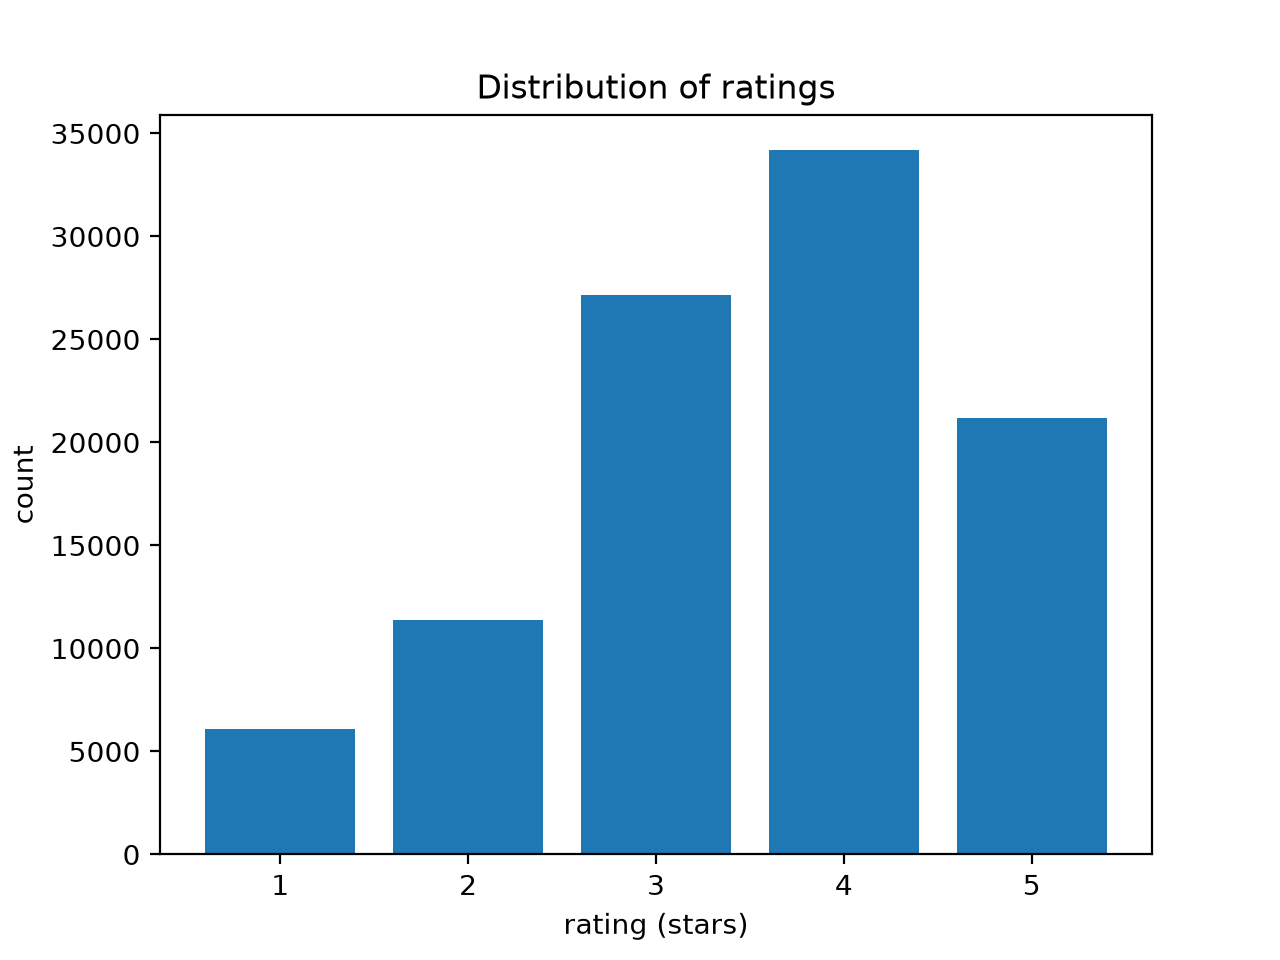
\includegraphics[width=0.48\textwidth]{rating_hist.png}\hfill
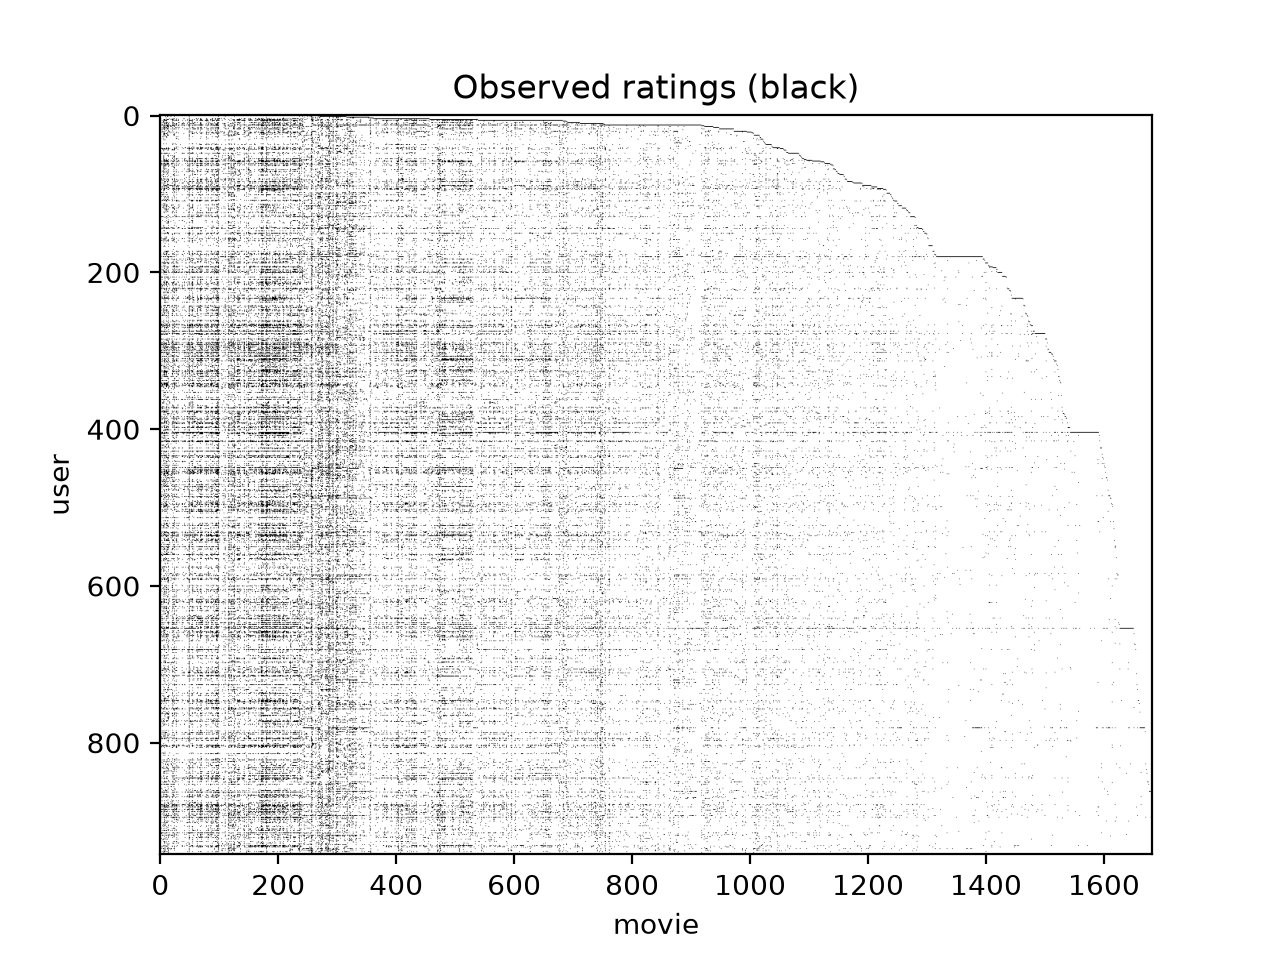
\includegraphics[width=0.48\textwidth]{sparsity.png}
\caption{Left: how many of each rating. Right: which entries of $R$ are known (black = known). Only about 6.3\% of $R$ is filled in.}
\label{fig:data}
\end{figure}

\section{Simulation Check}
\textbf{Setup.} We made a true rating matrix $R_{\text{true}}$ ($100\times80$) as the product of two random matrices with 3 columns, so its rank is exactly 3. We added noise with standard deviation 0.1 and kept only about 30\% of the entries (2281 known). Then we ran ALS with $k=3$, $\lambda=1$, for 50 sweeps. Seed: \texttt{np.random.default\_rng(0)}. Code: \texttt{src/simulation.py}.

\begin{table}[H]\centering\small
\begin{tabular}{lcc}
\toprule
What we checked & Expected & Got\\
\midrule
Top singular values & $100.11,\ 87.27,\ 85.28$ & $94.44,\ 82.95,\ 79.62$\\
4th singular value (rank 3) & 0 & 0\\
Hidden-entry RMSE, ALS & close to noise (0.1) & 0.147\\
Hidden-entry RMSE, fill with 0 then SVD & much worse & 1.394\\
Biggest gradient at a user update (Q2) & 0 & $5.7\times10^{-14}$\\
Smallest eigenvalue of $A$ (Q3) & $\ge\lambda=1$ & 1.832\\
Times $J$ went up (Q4) & 0 & 0 of 100\\
$J$: start, after 1 sweep, after 50 & going down & 14549, 4715, 547\\
\bottomrule
\end{tabular}
\end{table}
The estimated singular values are about 6\% low. That is expected: $\lambda$ pulls the vectors toward 0.

\begin{figure}[H]\centering
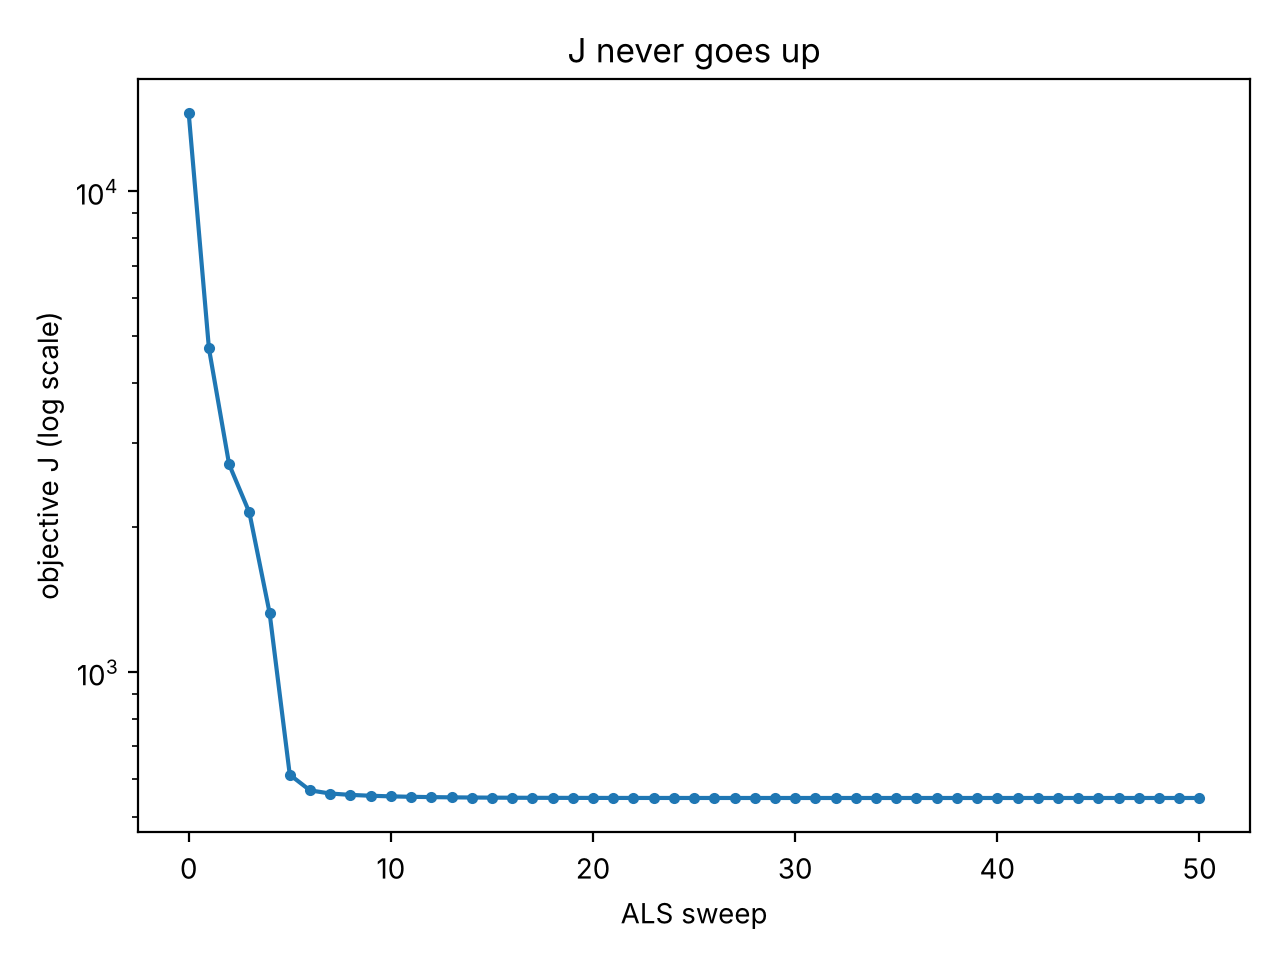
\includegraphics[width=0.55\textwidth]{sim_objective.png}
\caption{$J$ after each ALS sweep (log scale).}
\end{figure}

\textbf{What each result confirms.}
\begin{itemize}[nosep]
\item \textbf{Q1:} the coded $J$ only counts known entries, and ALS lowers it from 14549 to 547.
\item \textbf{Q2:} the gradient is 0 (up to rounding) at every user update, so the formula really finds the minimum.
\item \textbf{Q3:} every $A$ had all eigenvalues at least $\lambda$.
\item \textbf{Q4:} $J$ never went up.
\item \textbf{Q5:} ALS was about 10 times more accurate on hidden entries than filling with 0 and using the SVD.
\end{itemize}

\end{document}
